\documentclass[tikz]{standalone}

\begin{document}


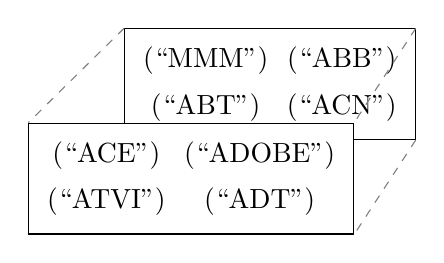
\begin{tikzpicture}
\def\xs{1} %shift in x direction
\def\ys{1.2} %shift in y direction
\def\nm{2} % number of 2d matrices in the 3d matrix


\matrix [draw, % for the rectangle border
         fill=white, % so that it is not transparent
         ampersand replacement=\&] %see explanation
(mm1)%give the matrix a name
at(-1* \xs, -1 * \ys) %shift the matrix
{
    \node {(``MMM'')}; \& \node {(``ABB'')};\\
    \node {(``ABT'')}; \& \node {(``ACN'')};\\
};

\matrix [draw, % for the rectangle border
         fill=white, % so that it is not transparent
         ampersand replacement=\&] %see explanation
(mm2)%give the matrix a name
at(-2* \xs, -2 * \ys) %shift the matrix
{
    \node {(``ACE'')}; \& \node {(``ADOBE'')};\\
    \node {(``ATVI'')}; \& \node {(``ADT'')};\\
};
\draw [dashed,gray](mm1.north west) -- (mm\nm.north west);
\draw [dashed,gray](mm1.north east) -- (mm\nm.north east);
\draw [dashed,gray](mm1.south east) -- (mm\nm.south east);


\end{tikzpicture}


\end{document}
